\documentclass[conference, 14pt]{IEEEtran}

\usepackage[utf8]{inputenc}
\usepackage[spanish]{babel}

\usepackage[T1]{fontenc}
\usepackage{lmodern}

\usepackage{csquotes}
\usepackage{amsmath,amssymb,amsfonts}
\usepackage[per-mode=fraction, inter-unit-product=\cdot, quotient-mode=fraction]{siunitx}
\usepackage[shortlabels]{enumitem}

\usepackage[style=ieee]{biblatex}
\addbibresource{proyecto-i.bib}

\usepackage{float}
\usepackage{graphicx}
\graphicspath{{./img}}

\usepackage{hyperref}
\hypersetup{colorlinks}

\begin{document}

\makeatletter
\newcommand{\linebreakand}{%
  \end{@IEEEauthorhalign}
  \hfill\mbox{}\par
  \mbox{}\hfill\begin{@IEEEauthorhalign}
}

\title{Proyecto I\\%
	\LARGE{Diseño de un ASIP de desencriptación mediante RSA}}

\author{
	\IEEEauthorblockN{Alejandro Soto Chacón, 2019008164}
	\IEEEauthorblockA{CE4301: Arquitectura de Computadores I \\
		Instituto Tecnológico de Costa Rica}}

\maketitle

\pagestyle{plain}
\thispagestyle{plain}

\section{Requerimientos}

Se desea construir un programa y herramientas asociadas para descifrar imágenes
	  en escala de grises que han sido cifradas píxel por píxel usando RSA dada
	  la pareja de llave privada $(n, d)$. El sistema implementado se adhiere
	  al RFC 3447: Public-Key Cryptography Standards (PKCS) \#1: RSA
	  Cryptography y la nomenclatura es la que esta norma dicta.

El sistema debe satisfacer los siguientes requerimientos generales:
\begin{itemize}

	\item Las imágenes son de tamaño 640x480 (resolución de facto utilizada
		desde hace varias décadas por sistemas de cómputo personal, ahora
		estandarizada como una resolución baseline en muchos sistemas de vídeo
		como "resolución VGA") sin cifrar y 640x960 cifradas, row-major.
	\item Cada píxel de plaintext es de 8 bits y cada píxel de ciphertext es de 16 bits.
	\item Los parámetros criptográficos tienen un rango máximo de 16 bits.
	\item La solución debe ser escrita en ensamblador e implementarse eficientemente
		para imágenes del tamaño deseado.
	\item Debe existir una forma cómoda al usuario de mostrar lado a lado en pantalla
		una imagen cifrada junto a su par descifrado.
	\item El formato de entrada de imágenes es de texto. Consiste de una
		secuencia de enteros de 8 bits sin signo separados por espacios. Cada
		píxel cifrado corresponde a dos consecutivos de estos enteros, el
		primero es el MSB y el segundo es el LSB. Es decir, el formato
		utilizado, con nomenclatura estándar de la industria, es 16bpp grayscale
		big-endian para el ciphertext.

\end{itemize}

\section{Propuestas de solución}

Se proponen y luego comparan dos soluciones distintas al problema planteado.

\subsection{RV64IM}

Esta solución utiliza RISC-V con base RV64I y extensión de multiplicación y
	  división entera para el cálculo de la operación módulo. La operación
	  central de exponenciación para descifrado no puede o debe realizarse de
	  la manera obvia, puesto que esto significaría un ineficiente y alto costo
	  computacional. En su lugar, se utiliza el algoritmo de exponenciación
	  modular de derecha a izquierda que se discutirá luego. Esta solución
	  recorre la imagen, descifrando los píxeles en su camino y repitiendo
	  hasta finalizar.

	  Véase la Figura \ref{fig:rv}.
	  \begin{figure}[H]
        \centering
		\caption{\label{fig:rv}Diagrama de flujo de alto nivel de la solución basada en RV64IM.}
		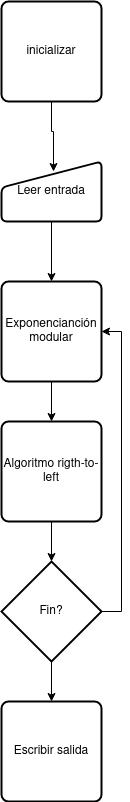
\includegraphics[width=.2\columnwidth]{diag-rv}
	  \end{figure}

\subsection{x86-64 con AVX2}

Esta es una solución vectorizada basada en el hardware disponible en sistemas
	  x86 contemporáneos. Se procesan 16 píxeles simultáneamente utilizando las
	  características de la extensión AVX2 que se discuten en la sección de
	  comparación. El algoritmo de división modular debe alterarse puesto que
	  sigue dependiendo de una operación módulo, la cual no existe en este
	  contexto. En su lugar, se utiliza el método de Granlund-Montgomery,
	  descrito posteriormente, que sí da lugar a esta posibilidad, volviéndose
	  un componente de programa que calcula la operación $a := ab \mod n$ para
	  una variable $a$. La mayoría del tiempo del programa se invierte en este
	  bucle. Como ese algoritmo produce un cociente, el resultado debe
	  ajustarse para obtener el módulo asociado.

	  Véase la Figura \ref{fig:x86}.
	  \begin{figure}[H]
        \centering
		\caption{\label{fig:x86}Diagrama de flujo de alto nivel de la solución basada en x86-64 con AVX2.}
		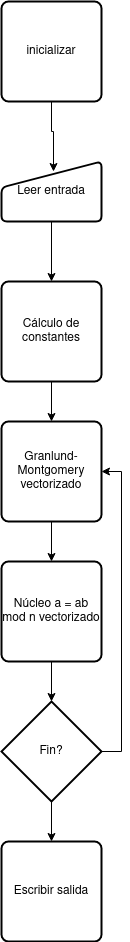
\includegraphics[width=.2\columnwidth]{diag-x86}
	  \end{figure}

\section{Comparación de propuestas}

Se comparan las dos propuestas para encontrar una solución a implementar.

\subsection{Opciones de ISA base}

Se comparan los ISAs base de las soluciones propuestas.

\subsubsection{RV64I}

	El ISA abierto RISC-V ha sido estabilizado recientemente y ha comenzado a
	  ver aplicaciones en la industria. RISC-V entra a competir inicialmente en
	  mercados empotrados y de aplicaciones específicas. El ISA base está
	  limitado a operaciones de aritmética, lógica, control de flujo y poco
	  más, siendo la intensión el extenderle con especificaciones adicionales,
	  denominadsa extensiones, a criterio del diseñador de hardware.

	  RISC-V posee ventajas respecto a un eventual diseño de hardware
	  customizado al problema particular. No obstante, esto último conlleva un
	  alto costo que, a saber, no ha sido considerado para el problema
	  planteado. Si se apunta a una implementación disponible existen algunas
	  opciones fuera del sector empotrado, como algunas de SiFive. Su diseño
	  RISC es capaz de potencialmente permitir un menor uso de potencia en la
	  implementación, 

	  Aunque esta solución podría también ser vectorizada, la extensión V se
	  encuentra en un estado de adopción muy temprano, aunque ya ha sido
	  congelada, y por tanto no se dispone de información para hacer
	  afirmaciones acerca de sus características en contextos de
	  implementación. Es posible amortiguar esta situación ligeramente ya que
	  RISC-V tiene casi el doble (31) de registros visibles de propósito
	  general que x86-64 (16) o incluso que la cantidad de píxeles procesados a
	  la vez por la implementación x86-64 con AVX2 (también 16).

\subsubsection{x86-64-v3}

	La larga y compleja historia de la línea x86 complica describir algún tipo
	de ISA base sobre el que se desea trabajar. Lo cierto es que la industria
	mantuvo por muchos años una clase de línea base de facto que lentamente se
	ha movido. Con el fin de estandarizar esta situación, recientemente se
	promueven varias versiones de x86-64, de entre las cuales x86-64-v3 es la
	seleccionada puesto que se requiere para la extensión AVX2. AVX2 ofrece 256
	bits en cada registro vectorial, extendiendo los 128 bits de SSE, y pueden
	segmentarse en 2 carriles de 128 bits enteros, 4 carriles de 64 bits
	(enteros o flotantes), 8 carriles de 32 bits (enteros o flotantes) y los
	menos comunes 16/32 carriles de 16/8 bits.

	  x86 es ubicuo en sistemas personales de escritorio y portátiles, en
	  computación de alto rendimiento, supercomputación y sistemas servidores.
	  Por esta razón, x86 tiene un precedente sólido y las características de
	  rendimiento de sus distintas implementaciones son bien conocidas. En
	  particular, las ofertas de rendimiento single-core de sistemas basados en
	  x86 siguen siendo de entre las mejores del mercado para muchos segmentos
	  de inversión. Además. Una desventaja en esta parte es que implementar
	  para x86 conlleva perder acceso a ciertos segmentos de cómputo, ya que su
	  simulación, emulación o virtualización no es nada trivial y no puede
	  realizarse en cualquier máquina de manera eficiente, no solo debido a su
	  diseño retroactivamente llamado CISC, sino también a la inmensa cantidad
	  de adiciones que se le han realizado a lo largo de más de 40 años.

	  Es importante recordar que esta misma abundancia de recursos, incluyendo
	  potencia, es la que le ha permitido alcanzar el rendimiento que tienen
	  sus implementaciones actuales, por lo que estos son factores negativos
	  respecto a x86 si se les debe tener más cautela.

\subsection{Técnicas de división de enteros}

La división de enteros está fuertemente ligada a las operaciones modulares que
	  se tendrán que implementar, indiferentemente de cual solución se escoge.
	  Existen diferencias concretas entre las soluciones propuestas en esta
	  materia.

\subsubsection{División por hardware}

La solución basada en RISC-V utiliza la extensión M\parencite[sec.~7]{rv-spec}
	  para multiplicación y división de enteros. Dividir en hardware es mucho
	  más eficiente que el equivalente en software que emiten algunos
	  compiladores para plataformas que no disponen de división por hardware.
	  RISC-V explícitamente soporta una instrucción \texttt{rem}, por lo que
	  puede calcular resultados modulares de baja magnitud sin necesidad de
	  ajustes adicionales.

\subsubsection{Método de Granlund-Montgomery}

Esta\parencite{divcnst} es una técnica que se puede aplicar cuando se conoce
que se realizarán muchas divisiones con el mismo divisor, pero el divisor no es
conocido antes de la ejecución del programa. En caso de que sí fuese conocido,
son posibles mejoras adicionales que escapan al objeto de discusión. El método
de Granlund-Montgomery reformula la división de dos enteros, con o sin signo,
en dos fases. En la primera se inicializan constantes, ejecutada una única vez,
y la segunda fase se realiza para cada división deseada. La segunda fase tiene
la propiedad de solamente utilizar multiplicación y corrimientos a la derecha.

En total, el costo de ambas fases es mayor que el de una sola división por
hardware, pero en código apropiadamente optimizado al caso este método puede
llegar a ser mucho más rápido, ya que las operaciones de segunda fase tienden a
tener un mejor perfil de paralelización en hardware que la división por
hardware. Concretamente, todas las revisiones de extensiones SIMD que se le han
incorporado a x86 carecen de división o módulo carril-con-carril, pero sí
tienen multiplicación vectorizada y corrimientos vectorizados, razón por la
cual este método se utiliza en la propuesta de solución con AVX2.

\section{Selección de solución}

Con base en los criterios analizados, la solución que puede ofrecer el mayor
rendimiento, y que además es más práctica para su distribución a usuarios
finales, es la opción x86-64 con AVX2, por lo que se implementa esta opción.

\section{Oportunidades de optimización}

Fuera de las opciones de diseño a gran escala, existen varias oportunidades de
optimización debido a las características de los requerimientos.

\subsection{Respecto a límites conocidos}

Como se conoce que cada píxel está asociado a dos bytes de ciphertext y un byte
de plaintext, esto puede tomarse en cuenta al momento de asignar registros y
distribuciones en memoria, como en efecto se hace. Para cada píxel se utiliza
uno de entre ocho carriles vectoriales de 32 bits para realizar todas las
operaciones, ya que este es el mínimo tamaño que se requiere para realizar una
multiplicación de dos enteros de 16 bits sin pérdida. Consideraciones parecidas
ocurren con los parámetros $n$ y $d$.

\subsection{Exponenciación modular}

Esta es una optimización sencilla que explota la propiedad de que, por ejemplo,
$a^{0b1101} \mod b$ = $a^{0b1000}a^{0b0100}a^{0b0001}a \mod b$ =
$a^{2^3}a^{2^2}a^{2^0} \mod b$ y además que $ac \mod m = (a \mod m)(c \mod m)
\mod m$, lo cual es sencillo y rápido de implementar eficientemente en código,
puesto que solo requiere relativamente pocos corrimientos y multiplicaciones
incluso para exponentes grandes.\parencite{modexp}

\subsection{Memoización de la relación ciphertext-plaintext}

Como solo hay 256 posibles resultados a descifrar, se mantiene una caché de
resultados ya calculados anteriormente, logrando que el ciclo de descifrado
solo tenga que ejecutarse 256 veces en el pero caso.

\printbibliography[title={Referencias}]

\end{document}
